\documentclass[11pt,a4paper]{article}
\usepackage[margin=2.3cm]{geometry}
\usepackage{amsmath,amssymb}
\usepackage{graphicx}
\usepackage{booktabs}
\usepackage{hyperref}
\usepackage{float}

\title{Rayleigh--Taylor instability with the SHAMROCK Godunov (RAMSES-like) solver}
\author{Run report}
\date{\today}

\newcommand{\commit}{75bf7ee}
\newcommand{\Lx}{0.5}
\newcommand{\Ly}{1.5}
\newcommand{\Lz}{0.5}
\newcommand{\yint}{0.75}
\newcommand{\nx}{32}
\newcommand{\ny}{96}
\newcommand{\nz}{32}
\newcommand{\dx}{1/64 \approx 0.0156}
\newcommand{\tend}{10}
\newcommand{\nframes}{51}
\newcommand{\sigmath}{0.647}
\newcommand{\tefold}{1.55}
\newcommand{\walltime}{about 15 minutes (903\,s spent in \texttt{evolve\_until}) on 4 CPU cores}
\newcommand{\morphology}{The perturbation is largest at the centre of the box, where it pushes upward, so the light fluid
forms a single bubble rising at $x = L_x/2$. The heavy fluid sinks as a spike at the periodic edge
$x = 0 \equiv L_x$. Until $t\approx 4$ the interface deformation stays small and sinusoidal (linear phase). By
$t\approx 7$ the bubble has a flat-topped, rounded cap and the spike has become narrow: the up--down
asymmetry between bubble and spike is the typical non-linear signature at moderate Atwood number. By
$t = 9$--$10$, shear along the flanks of the bubble rolls the heavy fluid into Kelvin--Helmholtz
vortices on both sides, giving the mushroom shape. At that point the bubble tip has reached
$y\approx 1.0$ and the spike $y\approx 0.42$, that is, an interface displacement of about $\pm 0.3$ from
$y_{\rm int} = 0.75$. With only 32 cells across the wavelength the interface is a few cells wide
and the roll-ups are smooth: numerical diffusion damps secondary instabilities at smaller scales.}
\newcommand{\growth}{Between $t=3$ and $t=7$ the kinetic energy grows exponentially. A least-squares fit gives
$2\sigma \approx 0.90$, so $\sigma_{\rm sim} \approx 0.45$, about $70\,\%$ of the ideal value. This lower
rate is expected for this setup: (i) the interface is spread over a few cells by the scheme, and
a diffuse interface lowers the effective Atwood number for $k\Delta x$ not small (here
$k\Delta x \approx 0.2$); (ii) the initial velocity field is not the pure linear eigenmode, so part
of the initial kinetic energy goes into stable and decaying components (which is why $E_{\rm kin}$
first decreases and oscillates (stable modes) until $t\approx 3$); (iii) the gas is weakly compressible, and the
perturbation amplitude is no longer small after $t\approx 6$. Saturation of the growth is visible after
$t\approx 8$, when the bubble enters the non-linear regime.}
\newcommand{\symmetry}{The asymmetry diagnostic is \emph{exactly zero} (to the last bit) at every one of the 51
outputs (Figure~\ref{fig:sym}). The solver therefore preserves the left--right mirror symmetry of
the problem perfectly, including through the non-linear Kelvin--Helmholtz roll-ups, where any
asymmetric round-off would normally be amplified. This is consistent with the symmetric van Leer
limiter and the bitwise-deterministic design of SHAMROCK.}
\newcommand{\energy}{The initial total energy is $E_{\rm tot}(0) \approx 2.375$, dominated by internal energy. During
the run, $\approx 1.03\times10^{-3}$ of gravitational potential energy is released as the heavy fluid
sinks. Of this, $\approx 0.96\times10^{-3}$ becomes kinetic energy and $\approx 6\times10^{-5}$ internal energy
(compression and numerical dissipation; this last number depends on the output time, see below). The total energy changes by only $-2.2\times10^{-6}$
relative to its initial value by $t=10$ (about $5\times10^{-3}$ of the energy actually exchanged). The
drift is smooth: it stays below $1.4\times10^{-7}$ during the linear phase and grows during the
non-linear phase. Some of it is expected, because $E_{\rm pot}$ in the diagnostic is computed at cell
centres while the scheme conserves its own discrete energy, and because the midpoint gravity
coupling is not exactly energy-conserving.

The variation panel (Figure~\ref{fig:energy}, right) also shows $E_{\rm int}$ and $E_{\rm pot}$ exchanging
$\sim 10^{-5}$ back and forth with a period of $\approx 2$ time units, in phase opposition, with no
signature in $E_{\rm tot}$. This is a global vertical breathing (gravity--acoustic) mode of the gas
column in the closed box. It is excited because the analytic hydrostatic profile, sampled at cell
centres with a density jump, is not exactly the discrete equilibrium of the scheme, and because the
initial $v_y$ field has a horizontally uniform part. It is small compared with the instability energy and
does not affect the RT growth.}
\newcommand{\summary}{\begin{itemize}
\item The Godunov (RAMSES-like) solver with HLLC, MUSCL--Hancock and constant external gravity
reproduces the expected Rayleigh--Taylor evolution qualitatively: a linear growth phase, a rising
bubble and a falling spike, then Kelvin--Helmholtz mushroom caps.
\item The measured linear growth rate, $\sigma \approx 0.45$, is $\approx 70\,\%$ of the sharp-interface,
incompressible prediction $\sqrt{\mathcal{A}gk} \approx 0.65$, which is reasonable at 32 cells per
wavelength.
\item Mirror symmetry is preserved exactly (zero to machine precision).
\item Total energy is conserved to $\sim 2\times10^{-6}$ (relative) over the run.
\item A convergence study (\texttt{base} = 16, 32, 64) would show whether the growth rate approaches
the theoretical value as resolution increases.
\end{itemize}}


\begin{document}
\maketitle

\begin{abstract}
This report describes the Rayleigh--Taylor (RT) instability test in
\texttt{examples/ramses/run\_rayleigh\_taylor.py} and shows the results of one run (SHAMROCK commit
\texttt{\commit}, AdaptiveCpp OpenMP backend, one CPU device with 4 cores). A heavy fluid sits on top of a
light one in a uniform gravity field. A small velocity perturbation at the interface grows into the
familiar rising bubbles and falling spikes, which then roll up into mushroom shapes. We also check
two properties the solver should keep: the left--right mirror symmetry of the setup, and the
conservation of total (kinetic + internal + gravitational) energy.
\end{abstract}

\section{Physical problem}

\subsection{Equations}
The gas follows the compressible Euler equations with an external gravitational acceleration
$\mathbf{g} = -g\,\mathbf{e}_y$:
\begin{align}
\partial_t \rho + \nabla\cdot(\rho\mathbf{v}) &= 0,\\
\partial_t (\rho\mathbf{v}) + \nabla\cdot(\rho\mathbf{v}\otimes\mathbf{v} + P\,\mathbb{I}) &= \rho\,\mathbf{g},\\
\partial_t (\rho e_{\rm tot}) + \nabla\cdot\big[(\rho e_{\rm tot} + P)\mathbf{v}\big] &= \rho\,\mathbf{v}\cdot\mathbf{g},
\end{align}
with $\rho e_{\rm tot} = \tfrac12\rho|\mathbf{v}|^2 + P/(\gamma-1)$ and an ideal-gas equation of
state with $\gamma = 1.4$.

\subsection{Why the interface is unstable}
When a heavier fluid rests on a lighter one in a gravity field, the stratification is in
equilibrium but that equilibrium is unstable. If the interface is displaced, heavy fluid that moves
down and light fluid that moves up release gravitational potential energy, and that energy feeds the
perturbation. Linear theory for two incompressible, inviscid fluids separated by a sharp interface
gives exponential growth $\delta \propto e^{\sigma t}$, with
\begin{equation}
\sigma = \sqrt{\mathcal{A}\,g\,k}, \qquad \mathcal{A} = \frac{\rho_h - \rho_l}{\rho_h + \rho_l},
\end{equation}
where $\mathcal{A}$ is the Atwood number and $k$ the wavenumber of the perturbation. In the
non-linear phase, light fluid rises as rounded \emph{bubbles} and heavy fluid falls as narrow
\emph{spikes}. Shear along the spike flanks then triggers secondary Kelvin--Helmholtz roll-ups,
which give the characteristic ``mushroom'' caps.

\section{Numerical setup}

\subsection{Initial conditions}
\begin{itemize}
\item Domain $[0,L_x]\times[0,L_y]\times[0,L_z]$ with $L_x = \Lx$, $L_y = \Ly$, $L_z = \Lz$, and the interface at
      $y_{\rm int} = L_y/2 = \yint$.
\item Density: $\rho_l = 1$ for $y \le y_{\rm int}$ (light fluid at the bottom), $\rho_h = 2$ above it (heavy
      fluid at the top), which gives $\mathcal{A} = 1/3$.
\item Pressure in hydrostatic equilibrium, continuous at the interface:
      $P(y) = P_0 - \rho\,g\,(y - y_{\rm int})$ with $P_0 = 2.5$ and $g = 0.1$.
\item Velocity perturbation, along $y$ only:
      \begin{equation}
      v_y = \frac{v_{\rm pert}}{4}\,\big[1+\cos(4\pi x')\big]\,\big[1+\cos(3\pi y')\big],\qquad
      x' = x - L_x/2,\; y' = y - y_{\rm int},
      \end{equation}
      with $v_{\rm pert} = 10^{-2}$. Along $x$ this is one wavelength, $\lambda = 0.5 = L_x$
      ($k = 4\pi$), centred on the middle of the box. All fields are evaluated at cell centres, so
      the initial state is exactly mirror-symmetric about $x = L_x/2$.
\end{itemize}
The flow is nearly incompressible: the sound speed $c_s = \sqrt{\gamma P/\rho}$ is about $1.3$--$1.9$,
while velocities stay of order $0.1$ or below. The problem is two-dimensional in nature. The $z$
direction is resolved only so that the patches stay compact, and nothing varies along $z$.

\subsection{Solver configuration}
\begin{table}[H]
\centering
\begin{tabular}{ll}
\toprule
Model & \texttt{Ramses} (Godunov finite volume on a block-structured grid), \texttt{f64\_3}\\
Grid & $\nx\times\ny\times\nz$ cells (blocks of $2^3$ cells), $\Delta x = \dx$\\
Riemann solver & HLLC\\
Reconstruction & MUSCL, symmetric van Leer slope limiter\\
Time integration & MUSCL--Hancock predictor with face time interpolation\\
CFL safety factor & $C_{\rm safe} = 0.8$\\
Gravity & \texttt{add\_ext\_force\_constant\_gravity}, $\mathbf{g} = (0,-0.1,0)$\\
Force coupling & midpoint rule (default; see below)\\
Boundaries & periodic in $x$, reflective in $y$ and $z$\\
Run & $t\in[0,\tend]$, \nframes\ outputs\\
\bottomrule
\end{tabular}
\end{table}

\paragraph{Gravity source term.} Each step, the constant acceleration is accumulated into an
external-acceleration field $\mathbf{a}_{\rm ext}$ (module \texttt{AddExtForceConstantGravity}). It is then
applied to the conservative variables after the flux update (module \texttt{ApplyExtForceGas}) with
a midpoint rule:
\begin{align}
\rho^{n+1/2} &= \rho^n + \tfrac{\Delta t}{2}\,\partial_t\rho, \qquad
(\rho\mathbf{v})^{n+1/2} = (\rho\mathbf{v})^n + \tfrac{\Delta t}{2}\,\partial_t(\rho\mathbf{v}),\\
(\rho\mathbf{v})^{n+1} &\mathrel{+}= \Delta t\,\rho^{n+1/2}\,\mathbf{a}_{\rm ext}, \qquad
(\rho e_{\rm tot})^{n+1} \mathrel{+}= \Delta t\,\mathbf{a}_{\rm ext}\cdot(\rho\mathbf{v})^{n+1/2}.
\end{align}
Here $\partial_t\rho$ and $\partial_t(\rho\mathbf{v})$ are the flux divergences of the current step,
so the source terms are evaluated at the half step, consistent with second-order accuracy in time.

\subsection{Diagnostics}
At each output the script records:
\begin{enumerate}
\item a density slice through the mid-plane $z = L_z/2$, sampled on an $\nx\times\ny$ grid (the frames of
      the GIF);
\item the \emph{mirror-symmetry error}
      $\max\, 2|\rho_{\rm left} - \rho_{\rm right}|/(|\rho_{\rm left}|+|\rho_{\rm right}|)$ between each point of
      that slice and its mirror image about $x = L_x/2$. The initial conditions and the
      equations are both symmetric, so in exact arithmetic this stays zero;
\item the volume-integrated energies $E_{\rm kin} = \int \tfrac12\rho v^2$,
      $E_{\rm int} = \int P/(\gamma-1)$ and $E_{\rm pot} = \int \rho g y$ (computed from cell centres), and their sum
      $E_{\rm tot}$, which should be conserved since the box is closed in $y$ and periodic in $x$.
\end{enumerate}

\section{Results}

\subsection{Morphology}
Figure~\ref{fig:snap} shows density snapshots, and the attached \texttt{rho\_rayleigh\_taylor.gif} shows the
whole evolution. \morphology

\begin{figure}[H]
\centering
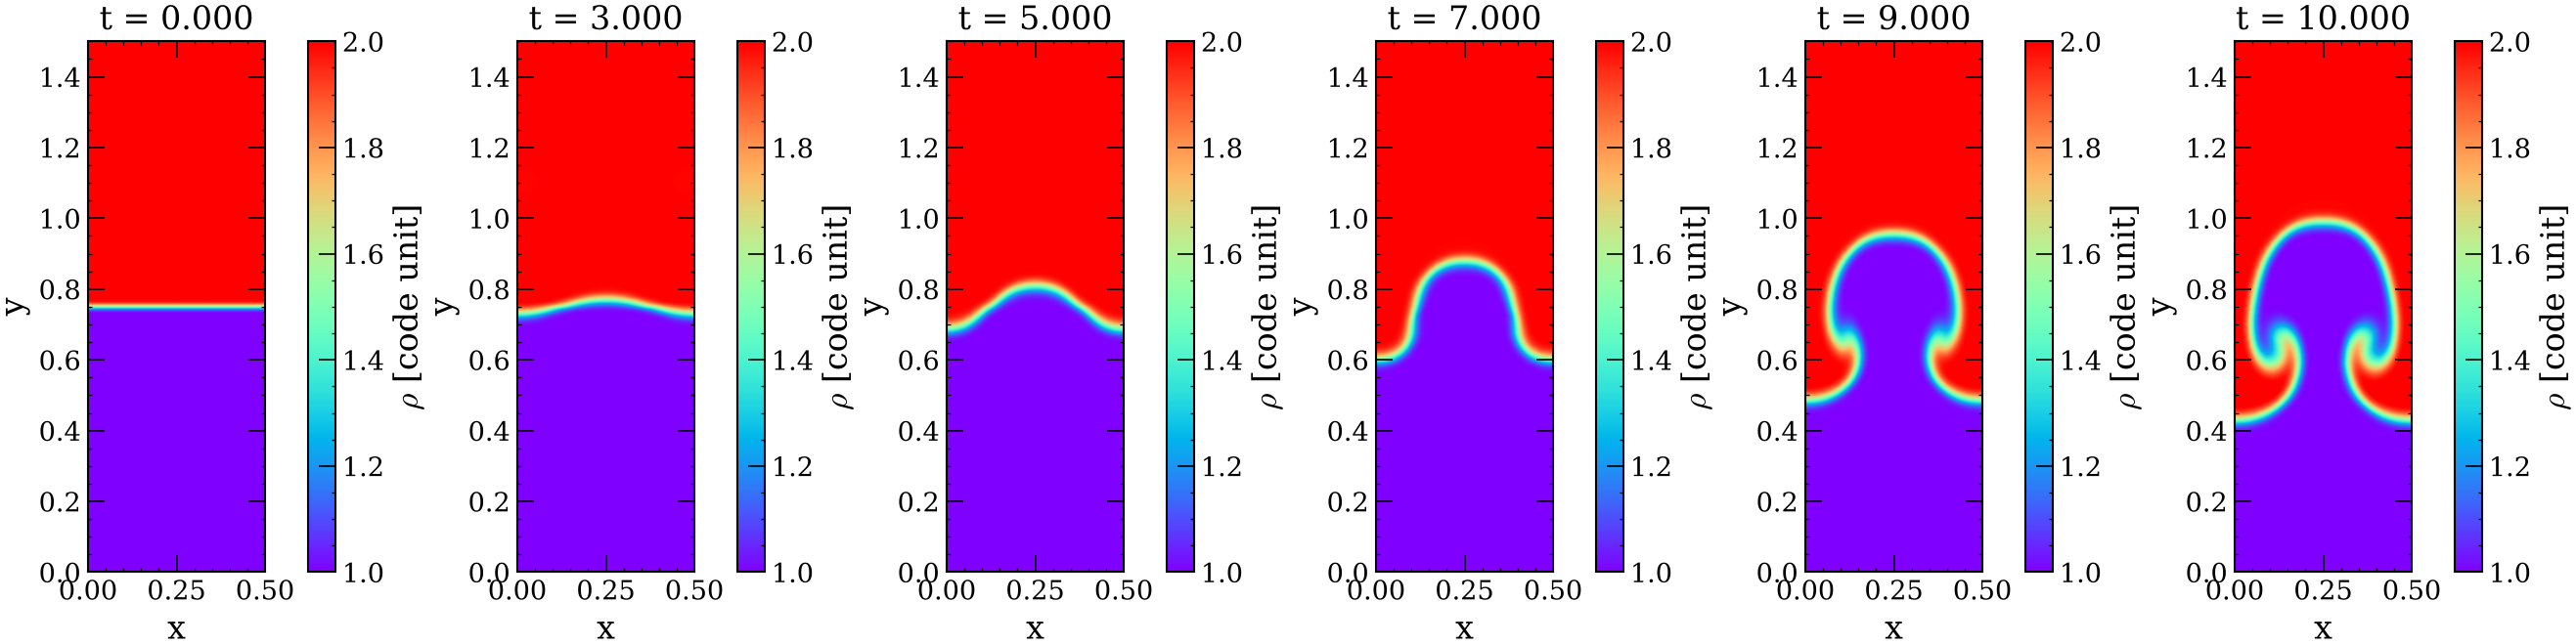
\includegraphics[width=\textwidth]{snapshots.png}
\caption{Density in the mid-plane $z=L_z/2$ at several times. Colour scale from $\rho=1$ (light fluid)
to $\rho=2$ (heavy fluid).}
\label{fig:snap}
\end{figure}

\subsection{Linear growth}
Linear theory predicts $\sigma = \sqrt{\mathcal{A} g k} = \sqrt{(1/3)(0.1)(4\pi)} \approx \sigmath$, that is, an
$e$-folding time of $\approx\tefold$. Figure~\ref{fig:growth} shows the total kinetic energy, which scales as the square of the
perturbation amplitude. \growth

\begin{figure}[H]
\centering
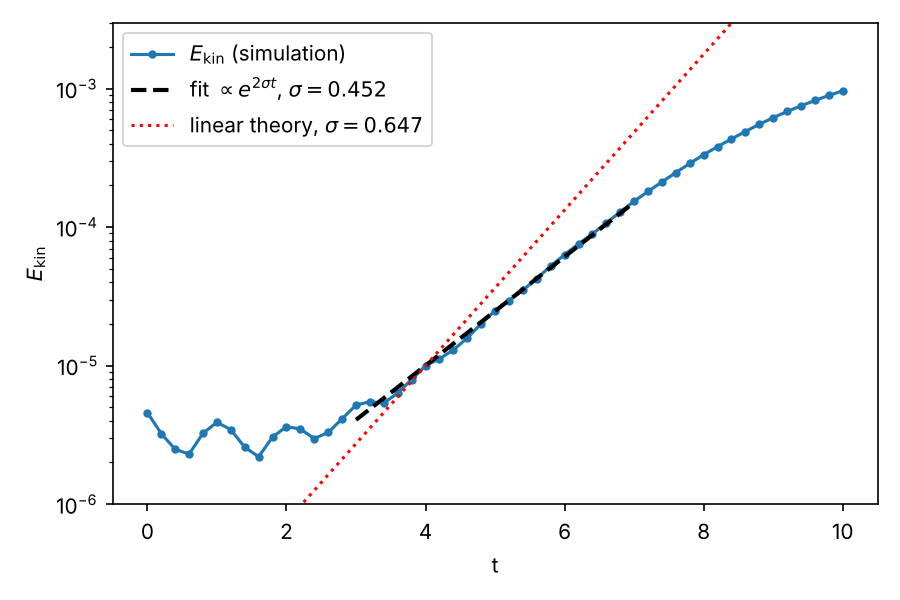
\includegraphics[width=0.7\textwidth]{growth.png}
\caption{Kinetic energy against time on a logarithmic scale, with a slope $e^{2\sigma t}$ (the
kinetic energy scales as amplitude squared) shown for reference.}
\label{fig:growth}
\end{figure}

\subsection{Mirror symmetry}
\symmetry

\begin{figure}[H]
\centering
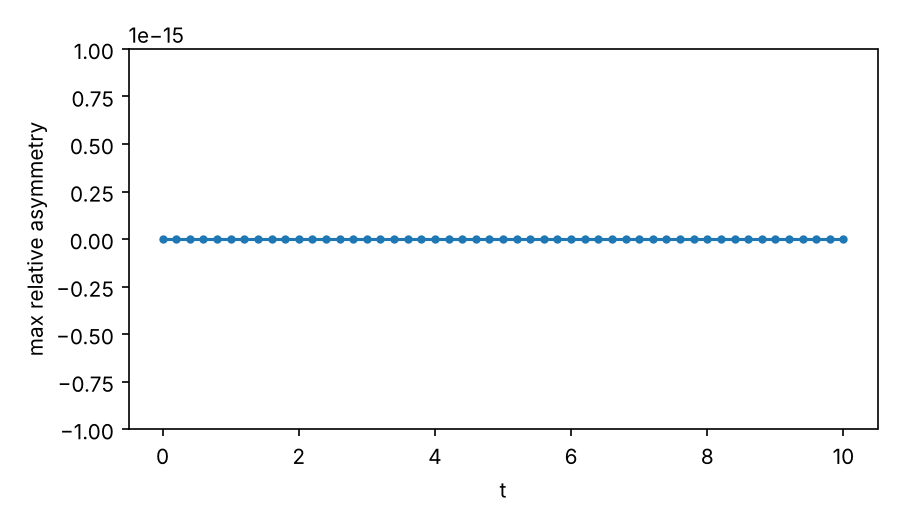
\includegraphics[width=0.65\textwidth]{symmetry.png}
\caption{Maximum relative left--right asymmetry of the density slice.}
\label{fig:sym}
\end{figure}

\subsection{Energy budget}
\energy

\begin{figure}[H]
\centering
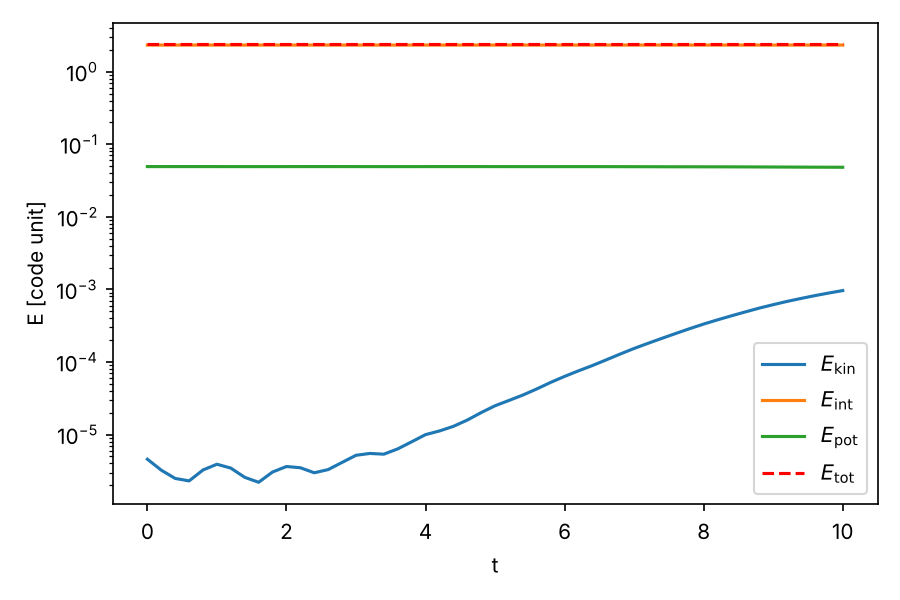
\includegraphics[width=0.49\textwidth]{energy.png}\hfill
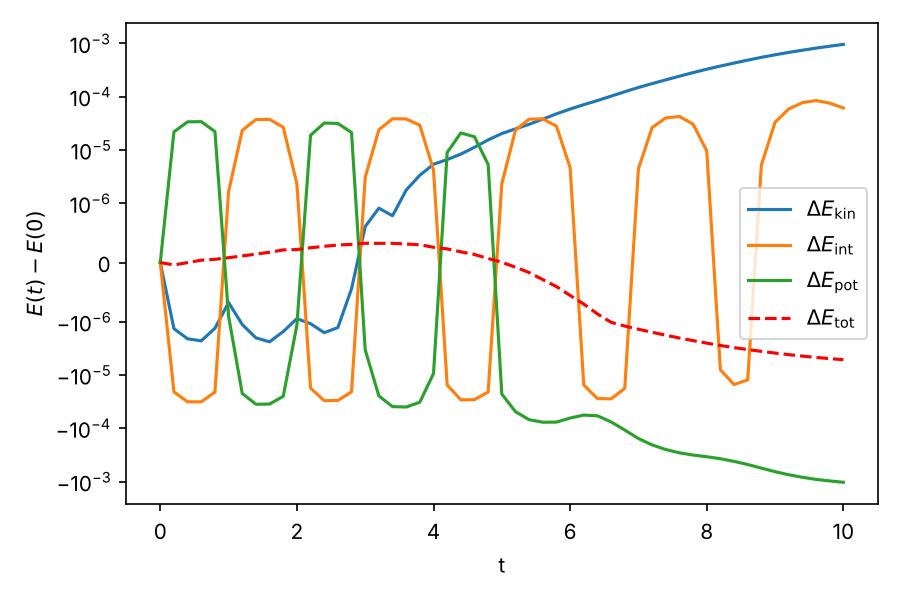
\includegraphics[width=0.49\textwidth]{energy_var.png}
\caption{Left: energy components. Right: variation with respect to $t=0$ (symlog scale).}
\label{fig:energy}
\end{figure}

\section{Summary}
\summary

\section*{Reproducing}
\begin{verbatim}
cd build
./shamenv_do shammake shamrock
./shamenv_do ./shamrock --sycl-cfg 0:0 --rscript \
    ../examples/ramses/run_rayleigh_taylor.py
\end{verbatim}
This run used \texttt{multy = 3} (the elongated $1\!:\!3$ box that the script suggests for a well-developed
instability) instead of the default \texttt{multy = 1}. Otherwise the parameters were unchanged.
Wall-clock time: \walltime.

\end{document}
